\documentclass[aspectratio=169]{beamer}
\usepackage{../../LaTex/simplemetropolis} % Load your custom style
% % Input encoding.
\usepackage[utf8]{inputenc} % For accents in spanish: transforms "á" into "\'a"
\usepackage[T1]{fontenc} % Output encoding. Use to avoid silly problems on the output.
                         % See: http://tex.stackexchange.com/questions/664/why-should-i-use-usepackaget1fontenc
\usepackage{lmodern} % Latin Modern fonts have broader support
% AMS packages
\usepackage{amsmath}
\usepackage{amsfonts}
\usepackage{amssymb}
\usepackage{amsthm}
\usepackage{bbm}
% Other maths packages
\usepackage{mathtools}
\usepackage{leftindex}
% Tables
\usepackage{booktabs}  % For professional tables
\usepackage{multirow}  % For multirow formatting
% Include animated gifs
\usepackage{animate}
% Hyperlink
\usepackage{hyperref}
\hypersetup{
	final,
    bookmarksnumbered=true,
    bookmarksopen=true,
    bookmarksopenlevel=0,
    unicode=false,          % non-Latin characters in Acrobat?s bookmarks
    pdftoolbar=true,        % show Acrobat?s toolbar?
    pdfmenubar=true,        % show Acrobat?s menu?
    pdffitwindow=false,     % window fit to page when opened
    pdftitle={Quantitative Methods For Humanities},    % title
    pdfdisplaydoctitle=true, %display document title instead of file name in title bar
    pdftoolbar=true,
    pdfmenubar=true,
    pdflang={English},
    pdfauthor={Abel Guada Azze},     % author
    pdfsubject={Quantitative Methods For Humanities},   % subject of the document
    pdfcreator={Abel Guada Azze},   % creator of the document
    pdfproducer={Abel Guada Azze}, % producer of the document
    pdfkeywords={Quantitative Methods} {R}, % list of keywords
    pdfnewwindow=true,      % links in new window
    breaklinks=true,
    hidelinks,
    colorlinks,
    linkcolor=CUNEFOrange,          % color of internal links (change box color with linkbordercolor)
    citecolor=black,        % color of links to bibliography
    filecolor=cyan,      % color of file links
    urlcolor=magenta           % color of external links
}
% Import icons
\usepackage{fontawesome}
\usepackage{tikz}
% \pgfplotsset{compat=1.18}
% \usepackage{tkz-euclide}
\usetikzlibrary{shapes,arrows,matrix,positioning,calc}
\newcommand{\tikzmark}[1]{\tikz[baseline,remember picture] \coordinate (#1) {};}
% Define colors
\definecolor{amber}{rgb}{1.0, 0.49, 0.0} % Normalized RGB
\definecolor{firebrick3}{RGB}{207, 33, 32} % 8-bit RGB
\definecolor{deepskyblue3}{RGB}{0, 155, 206} % 8-bit RGB
\definecolor{darkorange3}{RGB}{206, 102, 0} % 8-bit RGB
\definecolor{darkolivegreen3}{RGB}{163, 207, 91} % 8-bit RGB
\definecolor{purpleR}{RGB}{160, 32, 240}
% Customizable new commands
\usepackage{xparse}
% Plain macros
\newcommand{\R}{\mathbb{R}} % real number set
\newcommand{\N}{\mathbb{N}} % natural number set
\newcommand{\lp}{\left(} % left parenthesis
\newcommand{\rp}{\right)} % right parenthesis
\newcommand{\lb}{\left[} % left brackets
\newcommand{\rb}{\right]} % right brackets
\newcommand{\lc}{\left\{} % left curly brackets
\newcommand{\rc}{\right\}} % right curly brackets
\newcommand{\la}{\langle} % left angled brackets
\newcommand{\ra}{\rangle} % right angled brackets
\newcommand*{\defeq}{\mathrel{\vcenter{
                     \baselineskip0.5ex\lineskiplimit0pt
                     \hbox{\scriptsize.}\hbox{\scriptsize.}
                     }}%
                     =}
                     \newcommand{\Rcoef}{\textsf{R}^2} % Coefficient of determination
\newcommand{\adjRcoef}{\oline{\textsf{R}}^2} % Coefficient of determination
\newcommand{\SER}{\textsf{SER}} % Standard error of the regression
\newcommand{\SSR}{\textsf{SSR}} % Sum of squared residuals
\newcommand{\ESS}{\textsf{ESS}} % explained sum of squares
\newcommand{\TSS}{\textsf{TSS}} % total sum of squareds
% Macros with arguments
\newcommand{\lrav}[1]{\left|#1\right|} % absolute value
\newcommand{\wtilde}[1]{\widetilde{#1}}
\newcommand{\what}[1]{\widehat{#1}}
\newcommand{\oline}[1]{\overline{#1}}
\newcommand{\bs}[1]{\boldsymbol{#1}}
\newcommand{\lrp}[1]{\lp#1\rp} % left-right parenthesis
\newcommand{\lrb}[1]{\lb#1\rb} % left-right brackets
\newcommand{\lrc}[1]{\lc#1\rc} % left-right curly brackets
\newcommand{\lra}[1]{\la#1\ra} % left-right angled brackets
\RenewDocumentCommand{\Pr}{oe{_^}}{% Probability P
  \operatorname{\mathbb{P}}%
  \IfValueT{#2}{_{#2}}%
  ^{\IfValueTF{#3}{#3}{}}%
  \IfValueT{#1}{\lp #1 \rp}%
}
\NewDocumentCommand{\Esp}{oe{_^}}{%
  \operatorname{\mathbb{E}}%
  \IfValueT{#2}{_{#2}}%
  ^{\IfValueTF{#3}{#3}{}}%
  \IfValueT{#1}{\lb #1 \rb}%
}
\newcommand{\Var}[1]{\mathbb{V}ar\lb #1\rb} % variance
\newcommand{\Cov}[2]{\mathbb{C}ov\lb #1, #2\rb} % covariance
% Title, subtitle, author, and date
\title{Quantitative Methods for Humanities}
\subtitle{Introduction}
\author{}
\date{20254/2026}

\begin{document}

% Title page with custom background
{
    \usebackgroundtemplate{
\includegraphics[width=\paperwidth,height=\paperheight]{../../LaTex/img/title_page.png}}
    \begin{frame}[plain]
        % Logo in the upper left corner
        \vspace{-1cm} % Space between the logo and title
        {\hspace{-0.45cm} 
\includegraphics[width=2.5cm]{../../LaTex/img/logoCUNEF.png}} % Adjust the width as needed

        \vspace{1cm} % Space between the logo and title
        {\usebeamerfont{title}\usebeamercolor[fg]{title}\inserttitle\par}
        \vspace{-0.05cm} % Reduced space between title and separator
        \usebeamertemplate{title separator}
        \vspace{-0.05cm} % Reduced space between separator and subtitle
        {\usebeamerfont{subtitle}\usebeamercolor[fg]{subtitle}\insertsubtitle\par}
        \vfill
        {\usebeamerfont{date}\usebeamercolor[fg]{date}\insertdate\par}
    \end{frame}
}

%%%%%%%%%%%%%%%%%%%%%
% Organizational issues
%%%%%%%%%%%%%%%%%%%%
\begin{frame}
\frametitle{Organizational issues}
\begin{itemize}
    \item \textbf{E-mail:} \href{mailto:abel.guada@cunef.edu}{abel.guada@cunef.edu}
    \item \textbf{Office hours:} Monday and Wednesday 11:00-13:00, either in person or via Zoom (send an email beforehand!)
    \item \textbf{Software:} The course will use R for all computer-based exercises.
    \item \textbf{Evaluation:} 
    \begin{itemize}
        \item[$\bullet$] Continuous evaluation $40\%$
        \begin{itemize}
            \item[-] $5\%$ Quizzes at the end of each module
            \item[-] $5\%$ Practice about statistical software.
            \item[-] $15\%$ Midterm exam
            \item[-] $15\%$ R-based group project
        \end{itemize}
        \item[$\bullet$] Final exam $60\%$
        \begin{itemize}
            \item[-] Covers all topics 
            \item[-] Minimum grade is $5$!
        \end{itemize}
    \end{itemize}
\end{itemize}
\end{frame}

\begin{frame}
\frametitle{Organizational issues}
\begin{itemize}
    \item \textbf{Speaking in class}: You can only speak to contribute something to the class or to ask a question. People who disrupt the class will be expelled from the classroom. \medskip
    \item \textbf{Mobile phones}: They must remain in the backpack/bag during the class. \medskip
    \item \textbf{Laptops}: They can be used for taking notes and for practical class activities.\medskip
    \item \textbf{Punctuality}: You cannot enter the classrooms once the class has started.
\end{itemize}
\end{frame}

\begin{frame}
\frametitle{Organizational issues}
\centering
{\huge\alert{\textbf{EVERYTHING}} is in \alert{\textbf{CANVAS}}}
\vspace{1.5cm}

\hspace{0.3cm}
\begin{minipage}{0.3\textwidth}
\begin{itemize}
    \item[$\bullet$] Exam dates
    \item[$\bullet$] Project deadline
\end{itemize}
\end{minipage}
\begin{minipage}{0.3\textwidth}
\begin{itemize}
    \item[$\bullet$] Quizzes
    \item[$\bullet$] Teaching material
\end{itemize}
\end{minipage}
\begin{minipage}{0.3\textwidth}
\begin{itemize}
    \item[$\bullet$] Syllabus
    \item[$\bullet$] Announcements
\end{itemize}
\end{minipage}
% \begin{minipage}{0.45\textwidth}
%     \centering
%     
\includegraphics[width=0.5\textwidth]{../../LaTex/img/canvas_logo.png}
% \end{minipage}
\end{frame}

%%%%%%%%%%%%%%%%%%%%%
% Bibliography
%%%%%%%%%%%%%%%%%%%%

\begin{frame}
\frametitle{Main bibliography}
\begin{minipage}{0.65\textwidth}
    % \vspace{0.2cm}
    \href{https://press.princeton.edu/books/paperback/9780691175461/quantitative-social-science}{\textbf{Quantitative Social Science: An Introduction}} \\
    by Kosuke Imai.
    \vspace{0.2cm}
    
    \begin{itemize}
        \item \textbf{Hands-On Learning:} Illustrate concepts with real-world case studies.
        \item \textbf{Software compatibility:} Teaches data analysis using R.
        \item \textbf{\href{https://press.princeton.edu/student-resources/quantitative-social-science}{Rich Resources:}} Includes exercises, datasets, and online teaching materials.
        \item \textbf{Broad Applicability:} Relevant across sociology, economics, and politics fields.
    \end{itemize}
    \begin{center}
        \href{https://encuentra.cunef.edu/permalink/34CUNEF_INST/tmg4lg/alma991000470679408131}{Grab your copy!}
    \end{center}
    \end{minipage}
    \hspace{0.2cm}
    \begin{minipage}{0.3\textwidth}
        \centering
        
\includegraphics[width=\linewidth]{../../LaTex/img/Kosuke_book.jpg}
    \end{minipage}
\end{frame}

\begin{frame}
\frametitle{More bibliography... and even more in the syllabus}
\begin{minipage}{0.31\textwidth}
\begin{center}
    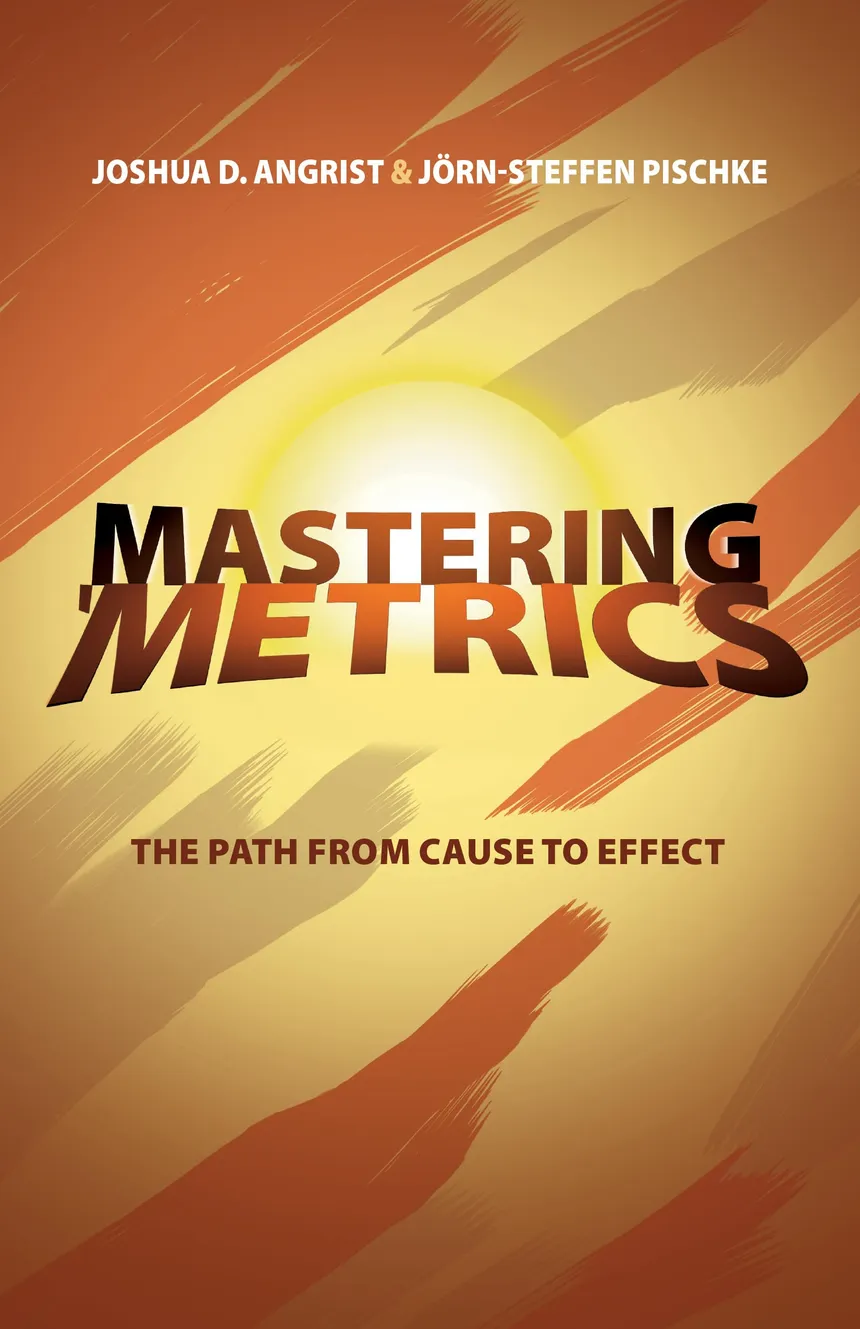
\includegraphics[width=\textwidth,height=0.7\textheight]{../../LaTex/img/mastering_metrics.png} \\[1em]
    {\small \href{https://encuentra.cunef.edu/permalink/34CUNEF_INST/tmg4lg/alma991000432079708131}{Grab your copy!}}
\end{center}
\end{minipage}
\hspace{0.25cm}
\begin{minipage}{0.31\textwidth}
\begin{center}
    
\includegraphics[width=\textwidth,height=0.7\textheight]{../../LaTex/img/social_research_method.png} \\[1em]
    {\small \href{https://encuentra.cunef.edu/permalink/34CUNEF_INST/tmg4lg/alma991000470679308131}{Grab your copy!}}
\end{center}
\end{minipage}
\hspace{0.25cm}
\begin{minipage}{0.31\textwidth}
\begin{center}
    
\includegraphics[width=\textwidth,height=0.7\textheight]{../../LaTex/img/wooldridge.png} \\[1em]
    {\small \href{https://encuentra.cunef.edu/permalink/34CUNEF_INST/1k9j0s0/alma991000155609708131}{Grab your copy!}}
\end{center}
\end{minipage}
\end{frame}

%%%%%%%%%%%%%%%%%%%%%
% Why study quantitative methods?
%%%%%%%%%%%%%%%%%%%%

\section{Why study Quantitative Methods?}

\begin{frame}
    \frametitle{What is Quantitative Methods?}
    
    \begin{coolblock}{Definition of Quantitative Methods}
    \textbf{Systematic approach} of \textbf{collecting and analyzing numerical data} to research.
    \end{coolblock}
    \vspace{0.8cm}

    \begin{itemize}
        \item \textbf{Tools of QM:} Statistics, mathematics, programming, data collection.
        \vspace{0.3cm}

        \item \textbf{Synonyms:} Quantitative research, numerical research, statistical methods, ... 
    \end{itemize}
    \vspace{0.5cm}
    
\end{frame}

\begin{frame}
    \frametitle{Common Characteristics of Quantitative Methods}
    \begin{itemize}
        \item Use of \textbf{measurable data} (e.g., percentages, averages, frequencies). \medskip
        \item Structured and standardized \textbf{data collection methodologies} like surveys or experiments. \medskip
        \item Focus on \textbf{causality} and \textbf{relationships} between variables. \medskip
        \item Deliver \textbf{insights} about larger populations out of \textbf{representative} samples.
    \end{itemize}
\end{frame}

\begin{frame}
\frametitle{Why to study Quantitative Methods}

    \begin{itemize}
        \item \textbf{It is the right moment:} Data + Computational revolution  \medskip
        \item \textbf{It is the right choice:} Data-driven decision making
    \end{itemize}
    \vspace{1cm}
    
    \begin{center}
        \begin{tcolorbox}[enhanced,sharp corners,
            width=8.5cm,
            colback=white,
            overlay={
                % Upper left corner (quotation mark)
                \node[anchor=north west,fill=white,draw=white,circle,inner sep=1pt] 
                at ([xshift=-0.17cm,yshift=0.2cm]frame.north west) {\faQuoteLeft};
                % Lower right corner (quotation mark)
                \node[anchor=south east,fill=white,draw=white,circle,inner sep=1pt] 
                at ([xshift=0.17cm,yshift=-0.2cm]frame.south east) {\faQuoteRight};
            }
            ]
            In God we trust; all others must bring data. \\
            \vspace{0cm}

            {\small - William Edwards Deming}
        \end{tcolorbox}
    \end{center}

\end{frame}


%%%%%%%%%%%%%%%%%%%%%
% Back Page
%%%%%%%%%%%%%%%%%%%%



\end{document}
